\documentclass[11pt]{amsart}
\usepackage{amsmath,amssymb,amsthm}
\usepackage{graphicx}
\usepackage{hyperref}
\usepackage{xcolor}

\theoremstyle{remark}
\newtheorem*{remark}{Remark}

\title{The Cone Program: A Roadmap}
\author{Jeremy Ebert}
\address{Independent researcher}
\date{October 5, 2026}

\begin{document}

\begin{abstract}
The discriminant-$12$ program studies a single geometric carrier ---
the cone $T^2=X^2+Y^2$, $T\ge 0$ --- which supports, without
modification, readings from elementary arithmetic, finite group
theory, Lorentzian geometry, bosonic quantum mechanics, and analytic
number theory.  This note maps those readings: what each paper in the
series establishes, how the pieces sit on the one cone, and what
remains honestly open.  It proves nothing new; its purpose is to let a
reader see the whole picture accurately, without overstatement.
\end{abstract}

\maketitle

\section{One carrier}

Everything in this program lives on one object: the cone
\[
T^2 = X^2 + Y^2, \qquad T \ge 0,
\]
with the AM--GM parametrization, for $x,y\ge 0$,
\[
T=\frac{x+y}{2}, \qquad X=\frac{x-y}{2}, \qquad Y=\sqrt{xy}.
\]
The multiplication table sits in the plane $Y=0$; its lift to the cone
is the substrate of the entire program.  Figure~\ref{fig:map} shows
the readings described below sitting on the one carrier.

The program's central claim, stated with care: each structure
described below is \emph{definable on this cone} --- no gluing, no
extra dimensions, no deformation of the carrier.  The cone carries
them all.  What is \emph{not} claimed is that these readings are
identified with one another.  The Lorentz group acting on the cone is
the Lorentz group of relativity; the $\mathfrak{su}(2)$ on the
fixed-$T$ rings is Schwinger's $\mathfrak{su}(2)$; the mod-$12$
arithmetic of the unit shell is mod-$12$ arithmetic.  The unity is in
the carrier, not in a claimed identification of the theories.  Every
paper in the series maintains this boundary, and this roadmap does
too.

\begin{figure}[t]
\centering
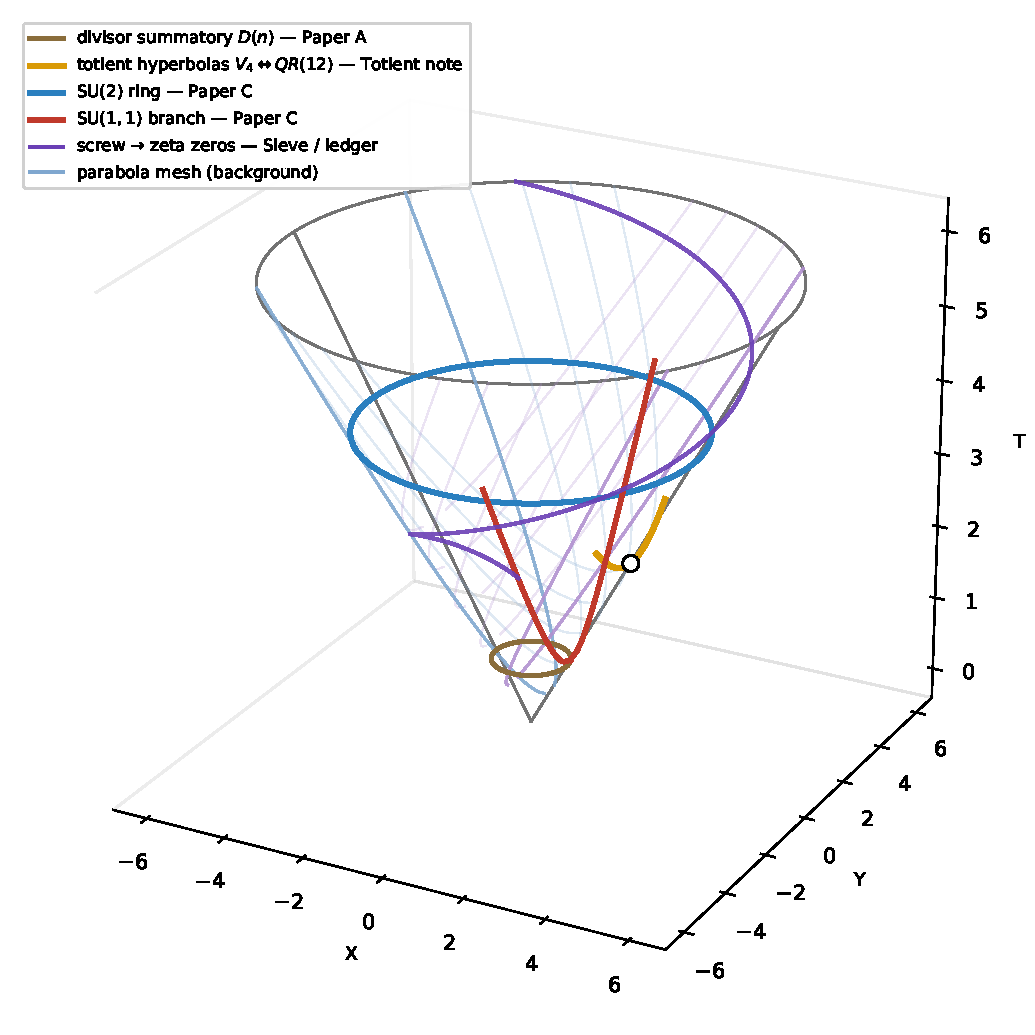
\includegraphics[width=0.92\textwidth]{fig_cone_roadmap.pdf}
\caption{Schematic map of the program's readings on the one cone:
the divisor-summatory base, the unit shell with its totient
hyperbolas, a fixed-$T$ $\mathrm{SU}(2)$ ring, a fixed-$X$
$\mathrm{SU}(1,1)$ branch, and the screw curve running toward the
analytic summit.  Schematic only; see the cited papers for the exact
statements.}
\label{fig:map}
\end{figure}

\section{The arithmetic base}

The program begins, in \cite{Ebert2026Table}, with the most elementary
object available: the multiplication table.  Linear conditions
$ax+by=c$ in factor coordinates cut the cone in complete conic
sections; constant products sit at reflected $Y$-levels with a common
Lorentz-type side view; the divisor summatory function
\[
D(n)=\sum_{k\le n} d(k)
\]
counts lattice points under the hyperbolas $xy\le n$; the summatory
region decomposes into diagonal gnomons.  A tangent construction
attaches to each factor level a unique anti-diagonal circle of radius
$u/2$.  The paper stops where geometry stops: no arithmetic or
operator identification is imported into the elementary proofs.

\section{The unit shell: where the program started}

The whole discriminant-$12$ idea grew out of a single picture,
recorded for the first time in \cite{Ebert2026Totient}.  For the units
$r\in U(12)=\{1,5,7,11\}$, the Paper-A sections $X=(r-1)/2$ are
hyperbolas $T^2-Y^2=((r-1)/2)^2$ passing through the unit-shell points
$(\pm(r-1)/2,\pm\sqrt r,(r+1)/2)$.  Their vertices $\{0,2,3,5\}$ and
their landing-circle radii $\{1,3,4,6\}$ both square to
$QR(12)=\{0,1,4,9\}$ modulo $12$ --- two bijections
$U(12)\to QR(12)$, one read at the vertices, one on the landing
circles.  The picture is exact, and it predates everything else in the
program: the unit shell came first, and the cone program was built
outward from it.

\section{The Lorentzian reading}

The cone $T^2=X^2+Y^2$ is the light cone of $(2+1)$-dimensional
Minkowski space, and the Lorentz group $SO(2,1)$ acts on it exactly as
the relativity group acts on spacetime --- this is the same group on
the same quadric, not an analogy.  \cite{Ebert2026EigenCoord}
classifies the signed cone cuts as Lorentz orbits and constructs
eigen-coordinates and power maps, separating intrinsic projective
self-maps of normalized orbit coordinates from equation-dependent
level-raising maps.  The fixed-$X$ hyperbolic sections of the
preceding section are the hyperbolic orbits of this action.

\section{The quantum reading}

Fix $T$: the circles $X^2+Y^2=\mathrm{const}$ carry Schwinger's
$\mathfrak{su}(2)$ --- two bosonic modes with total number conserved
and spin $j=T-\tfrac12$.  Fix $X$: the hyperbola branches carry the
two-mode $\mathfrak{su}(1,1)$ squeezing algebra, with number difference
conserved and Bargmann index $k=(|d|+1)/2$ for difference $d$.
\cite{Ebert2026Quantum} realizes both algebras on the cone with
Fock-state geometry and ladder operators, and proves the parity
selection rule and the operator revival identity for elliptic cuts.
\cite{Ebert2026NullDiamond} completes the picture at the Casimir
level: edge-centered spinor data, the primitive null diamond, and a
four-part taxonomy --- Casimir completion, null-edge geometry,
cyclotomic normalization, Boolean return --- that keeps the program's
distinct $V_4$ occurrences carefully apart.

A remark on loop quantum gravity, kept proportionate: the kinematic
variables of loop quantum gravity are $SU(2)$ holonomies, and its state
space is built from $SU(2)$ spin networks.  The $SU(2)$ on the cone's
fixed-$T$ rings is the same $SU(2)$ --- the same representation
theory, the same Casimir $j(j+1)$.  That is a shared kinematics, noted
here as a direction of travel, not a result.  Nothing about quantum
gravity is claimed.

\section{The analytic reading: toward the zeros}

The program's summit is analytic: the zeros of the Riemann zeta
function.  Two threads live on the cone here, at different levels of
maturity.

The sieve flow, recorded in \cite{Ebert2026Sieve}, is numerical
exploration: the primes $\le\sqrt N$ generate the exact
prime/composite bitmap on $[2,N]$ by the sieve of Eratosthenes, and
the zero spectrum reappears as fixed structure under the sieve lift at
every scale, with no Riemann-hypothesis input.  It is a measurement,
not a theorem, and is presented as one.

The screw thread is the program's main line: a screw function
overlaid on the cone, and the zeta function itself overlaid on the
cone, pursued through the discriminant-$12$ ledger toward a
Hilbert--P\'olya-type operator with the positivity certificate as the
gate.  The ledger records both progress and honest obstructions: the
continuum formulation cannot be closed unconditionally --- it is
RH-hard --- while the finite-scale formulation is unconditional.  The
open horizon has a name in the program: the \emph{selector},
whatever it is that chooses the zeros, which remains unidentified by
design rather than by oversight.

\section{What is established, and what is open}

\emph{Established} (proved in the series): the conic-section
classification and divisor-summatory geometry \cite{Ebert2026Table};
the $V_4\leftrightarrow QR(12)$ double bijection
\cite{Ebert2026Totient}; the Lorentz-orbit classification with
eigen-coordinates and power maps \cite{Ebert2026EigenCoord}; the
$\mathfrak{su}(2)$/$\mathfrak{su}(1,1)$ realizations with the parity
selection rule and revival identity \cite{Ebert2026Quantum}; the
Casimir completion and null-diamond taxonomy
\cite{Ebert2026NullDiamond}.

\emph{Exploratory} (numerical, not claimed as theorems): the
sieve-flow zero tracking \cite{Ebert2026Sieve}; the $T/D/A$ coloring of
the cone base; the mod-$0.5$ divisor detector.

\emph{Open}: the selector; the positivity certificate; every RH-hard
thread, so marked.

\section{Reading map}

\begin{center}
\begin{tabular}{lll}
Order & Paper & What it puts on the cone \\
\hline
1 & \cite{Ebert2026Table} & Conic sections; divisor summatory \\
2 & \cite{Ebert2026Totient} & The unit shell; $V_4\leftrightarrow QR(12)$ \\
3 & \cite{Ebert2026EigenCoord} & Lorentz orbits; power maps \\
4 & \cite{Ebert2026Quantum} & $\mathfrak{su}(2)$/$\mathfrak{su}(1,1)$; Fock geometry \\
5 & \cite{Ebert2026Cusp} & Cubic analog; cusp catastrophe; hysteresis \\
6 & \cite{Ebert2026Bicone} & Bicone $SO(4,2)$; hydrogen dipole; $\alpha$ from one line \\
7 & \cite{Ebert2026Kepler} & Kepler orbits as cone slices; dynamic slicing operator \\
8 & \cite{Ebert2026NullDiamond} & Casimir completion; null diamond \\
9 & \cite{Ebert2026Sieve} & Sieve flow; zero tracking (numerical) \\
\hline
\end{tabular}
\end{center}

The discriminant-$12$ return paper \cite{Ebert2026D12} is the
program's principal technical paper; the ledger continues the
main-line operator search.

\section*{Acknowledgment}
Large language model tools were used for drafting and structural editing.

\begin{thebibliography}{9}
\bibitem{Ebert2026Table} J.~Ebert, \emph{The Cutting Plane: Every Line
Through the Multiplication Table Is a Conic Section}, preprint (2026).
\bibitem{Ebert2026Totient} J.~Ebert, \emph{Totient Hyperbolas and the
$V_4\leftrightarrow QR(12)$ Bijection: A companion note to Paper A},
preprint (2026).
\bibitem{Ebert2026EigenCoord} J.~Ebert, \emph{Signed Cone Cuts as
Lorentz Orbits: Eigen-Coordinates and Power Maps}, preprint (2026).
\bibitem{Ebert2026Quantum} J.~Ebert, \emph{Two Oscillators, Two
Algebras: SU(2) and SU(1,1) Realizations of the Cone's Symmetry},
preprint (2026).
\bibitem{Ebert2026Cusp} J.~Ebert, \emph{The Cusp Instead of the Cone:
A Triple-Angle Analog of the AM--GM Circle via the Depressed Cubic,
and Its Catastrophe Dynamics}, preprint (2026).
\bibitem{Ebert2026Bicone} J.~Ebert, \emph{The Fine Structure Constant
from Bicone Geometry and One Spectral Line: Hydrogen dipole matrix
elements via $SO(4,2)$}, preprint (2026).
\bibitem{Ebert2026Kepler} J.~Ebert, \emph{The Dynamic Slicing Operator
on the AM--GM Cone: A Quadric Geometric Framework for Keplerian Orbits
and Perturbed Trajectories}, preprint (2026).
\bibitem{Ebert2026NullDiamond} J.~Ebert, \emph{Casimir Completion and
the Primitive Null Diamond}, preprint (2026).
\bibitem{Ebert2026Sieve} J.~Ebert, \emph{The Sieve-Flow Instrument:
Zeta Zeros from the Eratosthenes Renormalization}, preprint (2026).
\bibitem{Ebert2026D12} J.~Ebert, \emph{The Discriminant-$12$ Return:
From a Centered Cayley Selection to a Cyclotomic and Finite Arithmetic
Structure}, preprint (2026).
\end{thebibliography}

\end{document}
